% !TEX root = ../main.tex
\chapter{Background}
\label{Background}

\section*{Electricity as a Common Pool Resource}
A Common Pool Resource is a depletable resource which can be utilised by a group of people, characterised by a reduction in the availability of this resource as individuals withdraw or utilise this resource \cite{Ostrom:90}.  Electricity can be a Common Pool Resource if there exists a finite amount of electricity generation capacity. As users connect demand appliances to the generators, the availability of electricity supply for additional demand diminishes.

In developing communities with significant generation from renewable sources such as wind and solar, the availability of power can be highly variable between periods in time. This inherent volatility in the amount of available resource means that many communities can not be self-sustainable. By connecting multiple households and communities of consumer-providers (or \textit{Prosumer}) together, electricity generation and consumption can become diversified, increasing the sustainability of electricity access. Electricity in this case becomes a highly volatile Common Pool Resource.

Ostrom showed that Common Property Regimes (arrangements which resource consumers agree to) can be formed to maintain the Common Pool Resources by controlling the access to the resource \cite{Ostrom:90}. For this project, the arrangement will be the participation in a local micro-grid between a number Prosumers. The micro-grid will provide the infrastructure to allow electricity to be pooled as a Common Pool Resource, and will also provide the means to control the access to the resource.

\section*{Distributive Justice and Fair Allocation}
For the purpose of this project, a Micro-Grid is assumed to already exist and is being operated automatically by a third party. The Micro-Grid is also assumed to be able to enforce Prosumer contribution to the Common Pool and restrict its access. With the infrastructure for enforcing the \ac{CPR}, it is important to ensure that the allocation would be fair to encourage Prosumers to be part of the system. Being fair forms two of the necessary Ostrom's Principles for Enduring Institutions in a CPR \cite{Ostrom:90}. \\

\section*{Multi-Agent Simulation}
The simulation will be designed as a Multi-Agent System (MAS). MASes are particularly suited for this kind of model as Agents in MASes have three very important characteristics:
\begin{itemize}
	\item Autonomy: Agents act independently
	\item Local view: no Agent can see or manipulate the environment it is in
	\item Decentralised: no Agent can control the action of all Agents
\end{itemize}
In reality, individual households which are represented by Agents in the simulator all perform actions according to their individual and unique needs, and are not controlled by a third party. This makes Autonomy and Decentralisation a requirement for the Agents in the Simulator. Participants or households connected to the network can't directly control how other participants use or generate electricity for the Common Resource Pool, making it an requirement for the Agent to have a Localised view. 

\section*{Decentralised Community Energy Systems as a Holonic System}
A holonic system (or holarchy) is a system which is composed of interrelated subsystems or institution, each of which are in turn composed of "sub-subsystems"  or institutions and so on, recursively until reaching a lowest level of "elementary" subsystems. Each system, sub-system or institution has a well-defined set of goals or objectives which is achieved through enforcing a set of rules on its members or member-systems\cite{Pitt:Holonic_Institutions}. A holonic MAS is what will be utilised to simulate the dCES and associated CPR which allows the simulator to be scalable with any number of community participants and any number of communities. 

In the context of a rural dCES, a holonic system in this case would be composed of communities such as Districts, Provinces, Sectors which are composed of "sub-communities" such as Towns and Villages. The sub-communities would be composed of many "elementary" subsystems such as households, businesses and other points of connection for electricity. Each community or institution has the goal of gathering all generation from members, and subsequently fairly allocating electricity to all members. This goal would be achieved with the assumption that they are provided with the necessary infrastructure and powers for enforcing quotas and contribute to a common pool of electricity.

\subsection*{About Presage 2}
Presage 2 is a simulation platform for multi-nodal or Agent simulation of societies. The platform was built by Sam Macbeth and is currently maintained by PhD students within Imperial. This platform was chosen for the simulator as it enables the investigation of the impact of agent design (such as household behaviour), network properties (constraints on access) and the physical environment on individual agent behaviour and long-term global network performance \cite{Presage2-Desc:2015}. In the context of this Project, each Node or Agent can represent individuals, households, businesses or generators. 

In Presage 2, Agents are only allowed to act during increments of time steps, which makes the simulation a discrete time driven one. During each time step, all actions are required to be performed by Agents via \textit{Action Handlers} and \textit{Environment Services}. Figures \ref{fig:Presage_architecture} and \ref{fig:Presage_sim_architecture} illustrates the general and runtime architecture.

\begin{figure}[h!]
	\centering
	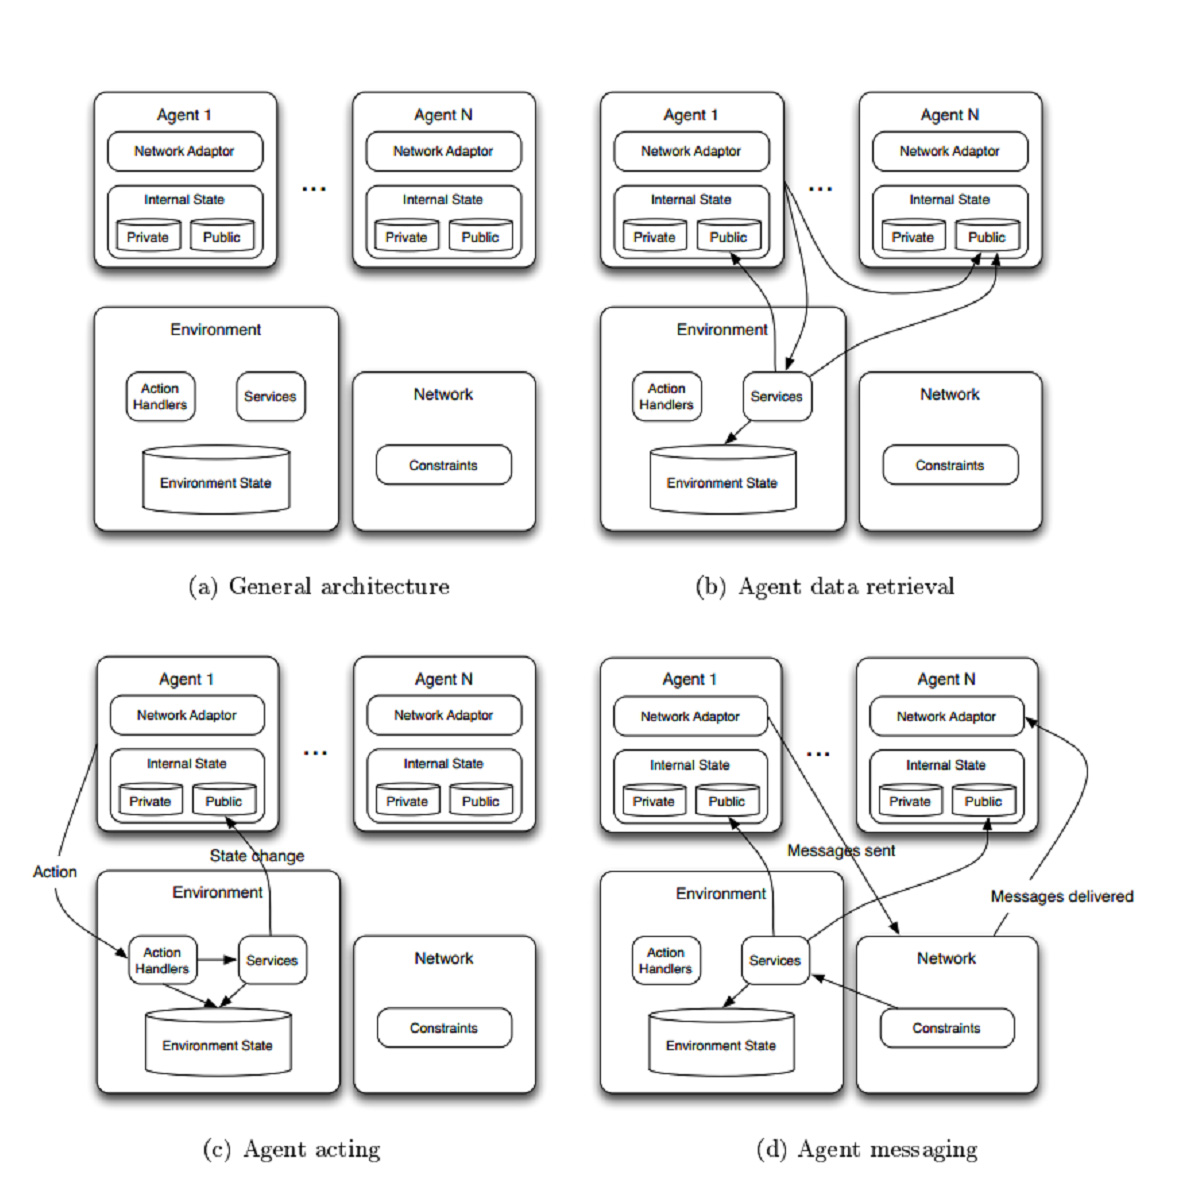
\includegraphics[scale=0.25]{Images/Presage.jpg}
	\caption{General Presage 2 architecture \cite{Presage_Kyoto:2015}}
	\label{fig:Presage_architecture}
\end{figure}

\begin{figure}[h!]
	\centering
	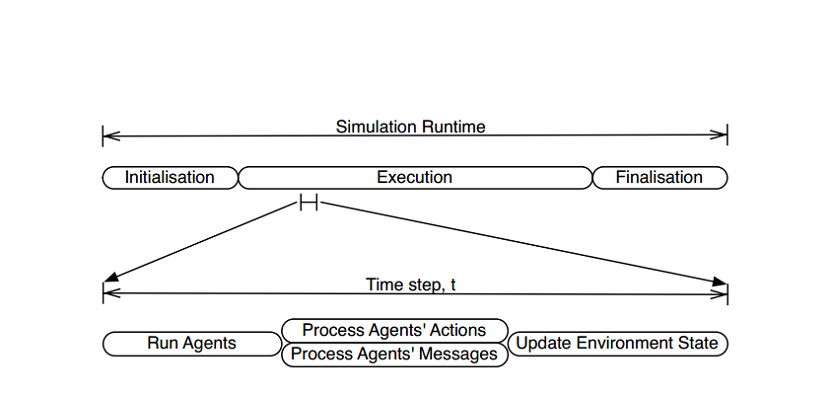
\includegraphics[scale=0.4]{Images/Presage2.jpg}
	\caption{Presage 2 simulation architecture \cite{Presage_Kyoto:2015}}
	\label{fig:Presage_sim_architecture}
\end{figure}

% \clearpage

